\section{Selection on Kin Cooperating Group Structure}

\begin{frame}{Design Objectives}
\begin{itemize}
\item selection for structure of kin cooperating group $\rightarrow$ expect fraternal transition to occur
\item scalable (i.e., distributed)
\item abstraction OK (i.e., ``realistic'' physics not reqd.)
\end{itemize}
\end{frame}

\begin{frame}{Resource Distribution}
\begin{figure}
\begin{columns}
\begin{column}{0.6\textwidth}
  \includegraphics<1>[width=\textwidth]{explanatory_sep/r-2.pdf}%
  \includegraphics<2>[width=\textwidth]{explanatory_sep/r-3.pdf}%
  \includegraphics<3>[width=\textwidth]{explanatory_sep/r-4.pdf}%
  \includegraphics<4>[width=\textwidth]{explanatory_sep/r-5.pdf}%
  \includegraphics<5>[width=\textwidth]{explanatory_sep/r-6.pdf}%
\end{column}
\begin{column}{0.2\textwidth}
\includegraphics<2>[width=\textwidth]{bolt.pdf}%
\end{column}
\end{columns}
\caption{TODO}
\end{figure}
\end{frame}

\begin{frame}{Resource Distribution}
\Large
\textbf{Problem:} how to alert neighbors to available resource?

\pause

\textbf{Solution:} activation-quiescence signaling

\end{frame}

\begin{frame}{Activation-Quiescence Signaling}
\begin{figure}
\begin{columns}
\begin{column}{0.45\textwidth}
  \includegraphics<1>[width=\textwidth]{explanatory_sep/r-2.pdf}%
  \includegraphics<2>[width=\textwidth]{explanatory_sep/r-3.pdf}%
  \includegraphics<3>[width=\textwidth]{explanatory_sep/r-4.pdf}%
  \includegraphics<4>[width=\textwidth]{explanatory_sep/r-5.pdf}%
  \includegraphics<5>[width=\textwidth]{explanatory_sep/r-6.pdf}%
\end{column}
\begin{column}{0.1\textwidth}
\includegraphics<2>[width=\textwidth]{bolt.pdf}%
\end{column}
\begin{column}{0.45\textwidth}

\foreach \n in {1,...,5}{%
  \includegraphics<\n>[width=\textwidth]{explanatory_sep/sig-\n-nohash.pdf}%
}%

\end{column}
\end{columns}
\caption{TODO}
\end{figure}
\end{frame}

\begin{frame}{Resource Distribution}
\Large
\textbf{Problem:} how to limit extent of signaling wave?

\normalsize

(i.e., to match limited extent of resource wave)

\Large

\pause

\textbf{Solution:} register cells into explicit cooperating groups called channels

\end{frame}


\begin{frame}{Same-channel Signaling Networks}

\begin{figure}

\begin{columns}
\begin{column}{0.45\textwidth}

  \foreach \n in {1,...,6}{%
  \includegraphics<\n>[width=\textwidth]{explanatory_sep/r-\n.pdf}%
  }%

\end{column}
\begin{column}{0.45\textwidth}

  \foreach \n in {1,...,6}{%
  \includegraphics<\n>[width=\textwidth]{explanatory_sep/s-\n.pdf}%
  }%

\end{column}
\begin{column}{0.1\textwidth}

  \foreach \n in {1,...,6}{%
  \includegraphics<\n>[width=\textwidth]{explanatory_sep/rs-\n.pdf}%
  }%

\end{column}
\end{columns}

\begin{columns}
\begin{column}{0.45\textwidth}
  \begin{subfigure}[b]{\textwidth}
  \caption{Resource}
  \end{subfigure}
\end{column}

\begin{column}{0.45\textwidth}
  \begin{subfigure}[b]{\textwidth}
  \caption{Channel map}
  \end{subfigure}
\end{column}

\begin{column}{0.1\textwidth}
  \begin{subfigure}[b]{\textwidth}
  \end{subfigure}
\end{column}

\end{columns}

\caption{
Frame-by-frame animation of a small same-channel network, activation signal, and resource wave interaction and effect on resource collection.
}

\end{figure}

\end{frame}

\begin{frame}{Same-channel Signaling Networks}

\begin{figure}

\begin{columns}
\begin{column}{0.45\textwidth}

  \foreach \n in {1,...,8}{%
  \includegraphics<\n>[width=\textwidth]{explanatory_sep/r-\n.pdf}%
  }%

\end{column}
\begin{column}{0.45\textwidth}

  \foreach \n in {1,...,8}{%
  \includegraphics<\n>[width=\textwidth]{explanatory_sep/m-\n.pdf}%
  }%

\end{column}
\begin{column}{0.1\textwidth}

  \foreach \n in {1,...,8}{%
  \includegraphics<\n>[width=\textwidth]{explanatory_sep/rm-\n.pdf}%
  }%

\end{column}
\end{columns}

\begin{columns}
\begin{column}{0.45\textwidth}
  \begin{subfigure}[b]{\textwidth}
  \caption{Resource}
  \end{subfigure}
\end{column}

\begin{column}{0.45\textwidth}
  \begin{subfigure}[b]{\textwidth}
  \caption{Channel map}
  \end{subfigure}
\end{column}

\begin{column}{0.1\textwidth}
  \begin{subfigure}[b]{\textwidth}
  \end{subfigure}
\end{column}

\end{columns}

\caption{
Frame-by-frame animation of a medium-sized same-channel network, activation signal, and resource wave interaction and effect on resource collection.
}

\end{figure}

\end{frame}

\begin{frame}{Same-channel Signaling Networks}

\begin{figure}

\begin{columns}
\begin{column}{0.45\textwidth}

  \foreach \n in {1,...,9}{%
  \includegraphics<\n>[width=\textwidth]{explanatory_sep/r-\n.pdf}%
  }%

\end{column}
\begin{column}{0.45\textwidth}

  \foreach \n in {1,...,9}{%
  \includegraphics<\n>[width=\textwidth]{explanatory_sep/l-\n.pdf}%
  }%

\end{column}
\begin{column}{0.1\textwidth}

  \foreach \n in {1,...,9}{%
  \includegraphics<\n>[width=\textwidth]{explanatory_sep/rl-\n.pdf}%
  }%

\end{column}
\end{columns}

\begin{columns}
\begin{column}{0.45\textwidth}
  \begin{subfigure}[b]{\textwidth}
  \caption{Resource}
  \end{subfigure}
\end{column}

\begin{column}{0.45\textwidth}
  \begin{subfigure}[b]{\textwidth}
  \caption{Channel map}
  \end{subfigure}
\end{column}

\begin{column}{0.1\textwidth}
  \begin{subfigure}[b]{\textwidth}
  \end{subfigure}
\end{column}

\end{columns}

\caption{
Frame-by-frame animation of a large same-channel network, activation signal, and resource wave interaction and effect on resource collection.
}

\end{figure}

\end{frame}

\begin{frame}{Same-channel Signaling Networks}

\Large
\textbf{Problem:} how to define same-channel signaling groups?

\pause

\textbf{Solution:} make channel-membership inherited

\normalsize
(with possibility of setting offspring to new channel)

\end{frame}

\begin{frame}{Channel Inheritance}
  \vspace{8ex}
  \begin{figure}
\begin{columns}
  \begin{column}{0.5\textwidth}
    \colorbox{extralightgray}{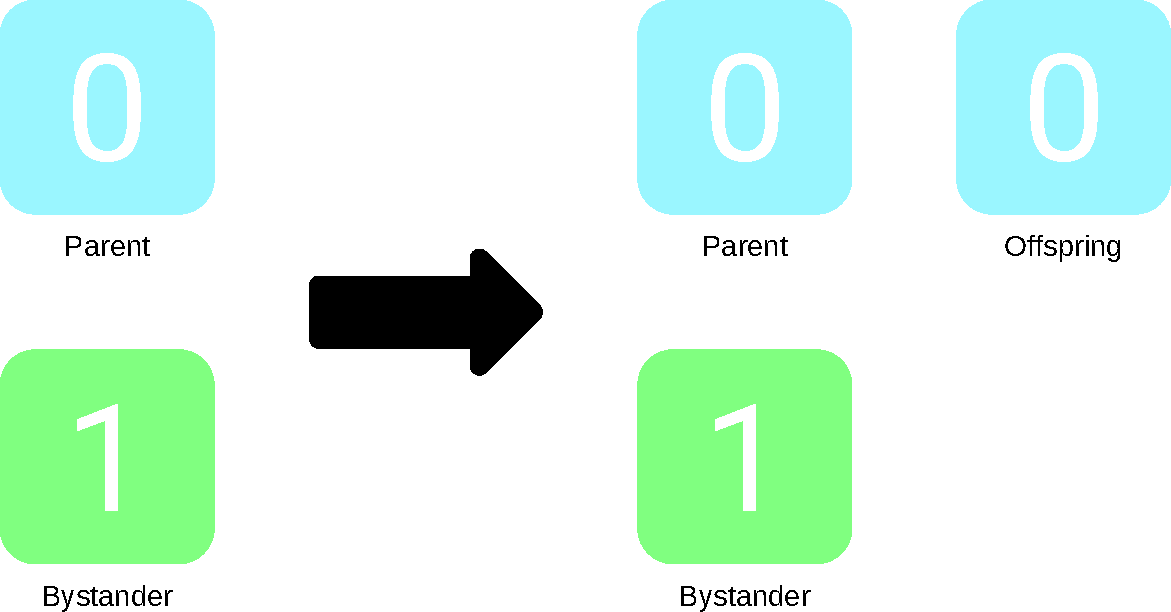
\includegraphics[width=\textwidth]{same_channel_offspring}}
  \end{column}%
  \begin{column}{0.5\textwidth}
    \colorbox{extralightgray}{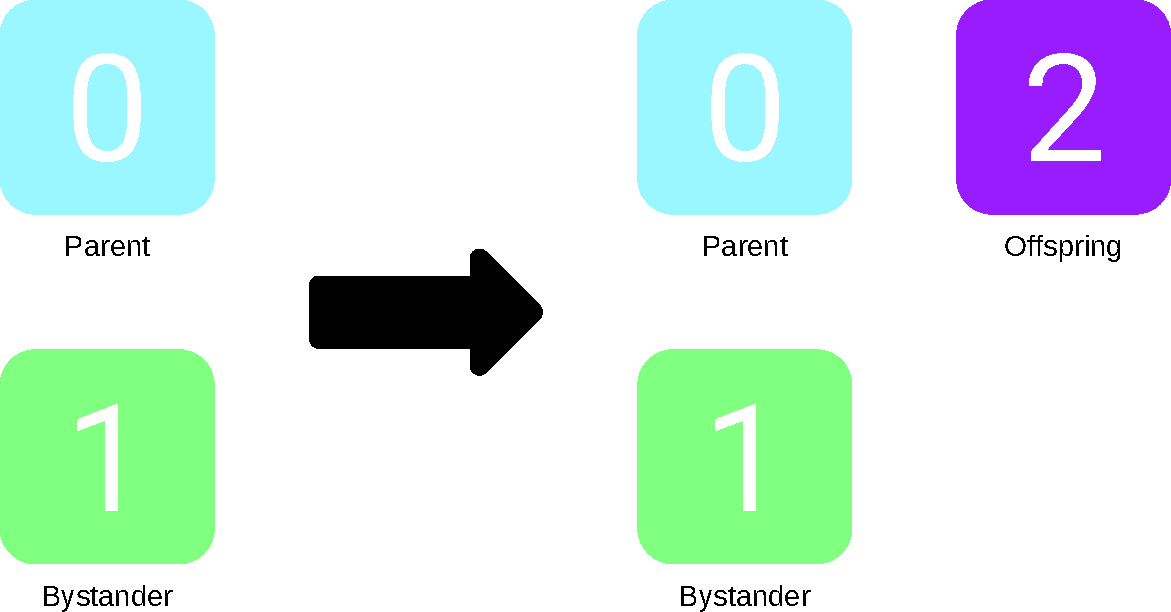
\includegraphics[width=\textwidth]{new_channel_offspring}}
  \end{column}%
\end{columns}%
\begin{columns}
  \begin{column}{0.5\textwidth}
    \begin{subfigure}[b]{\textwidth}
    \caption{Offspring inherits channel ID from parent.}
    \end{subfigure}
  \end{column}%
  \begin{column}{0.5\textwidth}
    \begin{subfigure}[b]{\textwidth}
    \caption{Offspring assigned new, unique channel ID.}
    \end{subfigure}
  \end{column}%
\end{columns}%
\caption{The two possible channel inheritance outcomes.}
\end{figure}

\end{frame}

\begin{frame}{Excluded Channel Dynamics}
  \vspace{6.6ex}
  \begin{figure}
\begin{columns}
  \begin{column}{0.5\textwidth}
\colorbox{extralightgray}{\hspace{0.136\textwidth}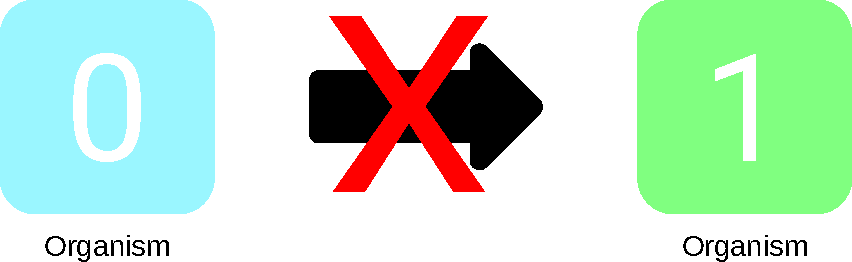
\includegraphics[width=0.728\textwidth,trim= 0 -83 0 -83]{plastic_channel}\hspace{0.136\textwidth}}
  \end{column}%
  \begin{column}{0.5\textwidth}%
\colorbox{extralightgray}{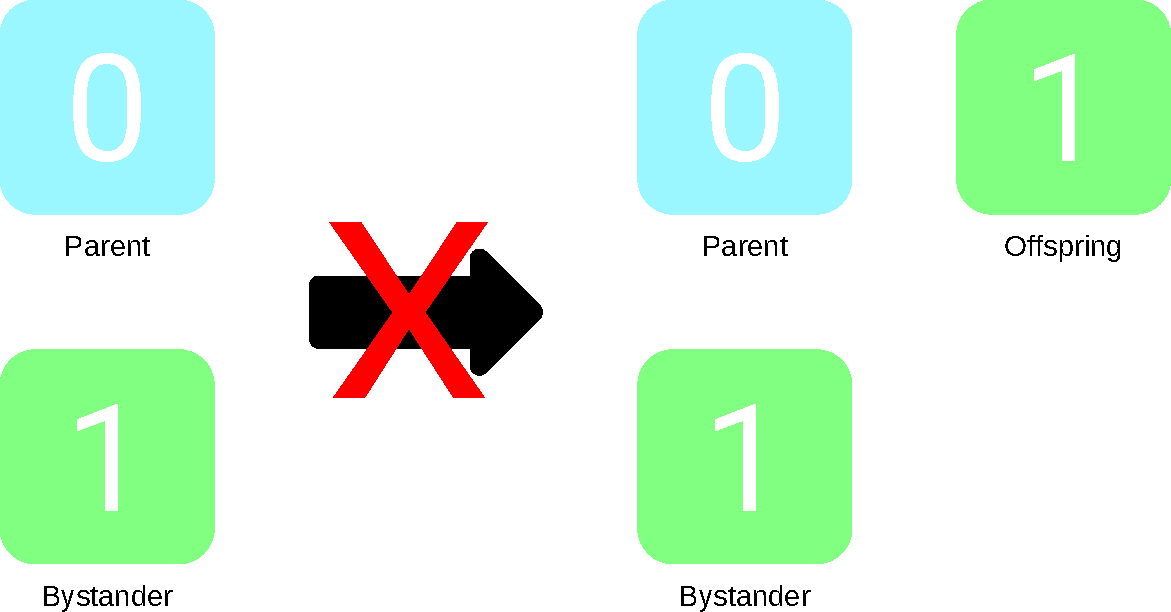
\includegraphics[width=\textwidth]{channel_collision_offspring}}
  \end{column}
\end{columns}%
\begin{columns}
  \begin{column}{0.5\textwidth}
    \begin{subfigure}[b]{\textwidth}
    \caption{during-lifetime channel change}
    \end{subfigure}
  \end{column}
  \begin{column}{0.5\textwidth}
    \begin{subfigure}[b]{\textwidth}
    \caption{non-inherited channel match\footnotemark}
    \end{subfigure}
  \end{column}
\end{columns}
\caption{Illustration of excluded channel dynamics.}
\end{figure}
\footnotetext{infrequent, non-inducible}

\end{frame}

\begin{frame}{Channels, Signals, \& Resource}
key idea: selection on regulation of same-channel group size \& shape
\pause
\begin{itemize}[<+->]
  \item too small: low resource-collection rate
  \item too big: net negative resource collection due to erroneous activation
\end{itemize}

\end{frame}

\begin{frame}{Selection for Resource-Sharing + Reproductive Division of Labor}

\begin{figure}
\begin{columns}
\begin{column}{0.5\textwidth}
  
\includegraphics[width=\textwidth]{channelviz/channelviz-clump-crop}
\end{column}
\begin{column}{0.5\textwidth}
  
\includegraphics[width=\textwidth]{channelviz/channelviz-clump2-crop}
\end{column}
\end{columns}
\caption{A juxtaposition of two (competing) clumps.}
\end{figure}

\end{frame}
